\section{Introduction}
\label{sec:introduction}

The development of Generative AI (GenAI) Large Language Models (LLMs), coupled with the easy API based accessibility of powerful models with hundreds of billions of parameters,  has brought significant advancements in artificial intelligence, allowing systems to generate human-like content across various mediums, including text, images, and code \cite{intro2LLM}. Meanwhile, digital chip design is becoming increasingly complex, requiring management of millions to billions of transistors while optimizing performance, power consumption, and area. Furthermore, it demands precise coordination of design factors such as timing, signal integrity, and manufacturability, all within stringent time-to-market constraints. Recent research has investigated the application of LLMs in digital design, particularly in generating hardware description languages (HDLs) such as Verilog from natural language design descriptions. The use of LLMs in VLSI system design is part of a larger effort by the research community to improve designer productivity, and costs needed to realize complex System-on-Chips (SoCs) \cite{ajayi2019openroad}.

In the last year or so, agentic AI workflows have emerged, where autonomous AI agents perform specific tasks within defined parameters \cite{promptengineering2024}. Agentic AI systems are defined by their capacity to take actions that consistently work toward achieving goals over time, even when their behavior is not pre-programmed in advance. Agents utilize an LLM to reason and determine the sequence of actions to take. Figure \ref{fig:agentic_overview} shows the high-level outline of an agentic workflow.  These workflows are increasingly used in software design to automate tasks such as code generation, debugging, and testing, thus improving development speed and minimizing human error. While agentic AI workflows have proven effective in software code generation, applying these techniques to hardware design presents additional complexities. This is due to the diverse range of tools required to meet functional and timing correctness, in addition to physical constraints in hardware systems.


\begin{figure}[htbp]
	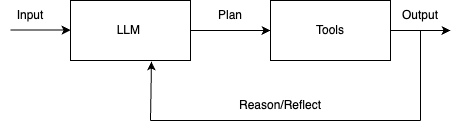
\includegraphics[width=0.45\textwidth]{figs/agentic_overview.png}
	\caption{Agentic AI workflow involves an iterative process involving one or more LLMs for reasoning, and planning, and one or more external tools to execute actions. The input could be a design specification in natural language, or a behavioral description in an HDL. The output could be HDL, netlist, or a GDS layout.
}
	\label{fig:agentic_overview}
\end{figure}

In this paper, we propose AiEDA, an agentic design flow framework in the design of a digital ASIC system from concept to GDSII using an open source tool flow. Our premise is that the use of agentic AI workflows in digital design would greatly increase designer productivity, enabling rapid implementation of design ideas that integrate a number of different design tools, to generate a full system design is ready to be fabricated. We demonstrate the use of the proposed framework, via the design of a ultra low power digital ASIC for KeyWord Spotting(KWS) architecture. 

The paper is organized as follows. In Section \ref{sec:related_work}, we briefly review the literature on the use of generative AI in hardware design. 
%In Section \ref{sec:background}, we provide a background on agentic AI workflows and the open source digital design tool flow considered in this work. 
In Section \ref{sec:agentic} , we describe AiEDA, our proposed agentic AI design framework. In Sections \ref{sec:system_design} and Sections \ref{sec:preliminary_evaluation} we present the KWS architecture, and our initial results in using AiEDA to design it. In Section \ref{sec:discussion}, we discuss the broader applicability of agentic flow in digital system design, the open research questions that need to be addressed, and our current research efforts in this direction. Section \ref{sec:conclusions} concludes the paper.

